
\begin{frame}
    \myheading{Module 7.6: Contractive Autoencoders }
\end{frame}

% Module 6: Contractive autoencoders starts here (Slide 46 to 51) 

\begin{frame}
  \begin{columns}
    \column{0.5\textwidth}
    \begin{overlayarea}{\textwidth}{\textheight}
        \begin{itemize}[]\justifying
            \item<1-> A contractive autoencoder also tries to prevent an overcomplete autoencoder from learning the identity function.
            \item<2-> It does so by adding the following regularization term to the loss function\\
            \[
                \Omega(\theta) = \|J_{\textbf{x}}(\mathbf{h})\|_F^2
            \]
            \item<3->[] where $J_{\textbf{x}}(\mathbf{h})$ is the Jacobian of the encoder.
            \item<4-> Let us see what it looks like.
        \end{itemize}
    \end{overlayarea}

    \column{0.5\textwidth}
    \begin{overlayarea}{\textwidth}{\textheight}
        \only<1->{
            \hspace{-0.3cm}
            % \tikzstyle{input_neuron}=[circle,draw=red!50,fill=red!10,thick,minimum size=6mm]
\tikzstyle{hidden_neuron}=[circle,draw=blue!50,fill=cyan!10,thick,minimum size=6mm]
\tikzstyle{output_neuron}=[circle,draw=green!50,fill=green!10,thick,minimum size=6mm]
\tikzstyle{cpy_neuron}=[circle,draw=red!50,fill=red!50,thick,minimum size=6mm]
\tikzstyle{input}=[circle,draw=black!50,fill=black!20,thick,minimum size=6mm]

\begin{center}
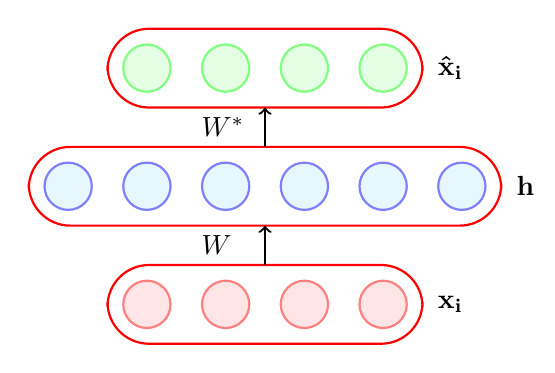
\begin{tikzpicture}

\node [input_neuron] (neuron01) at (8.5,4.5) {};
\node [input_neuron] (neuron02) at (9.5,4.5){};
\node [input_neuron] (neuron03) at (10.5,4.5) {};
\node [input_neuron] (neuron04) at (11.5,4.5) {};
\node [hidden_neuron] (neuron51) at (7.5,6) {} ;
\node [hidden_neuron] (neuron52) at (8.5,6)  {};
\node [hidden_neuron] (neuron53) at (9.5,6)  {};
\node [hidden_neuron] (neuron54) at (10.5,6)  {};
\node [hidden_neuron] (neuron55) at (11.5,6)  {};
\node [hidden_neuron] (neuron56) at (12.5,6)  {};

\node [output_neuron] (neuron11) at (8.5,7.5)  {};
\node [output_neuron] (neuron12) at (9.5,7.5)  {};
\node [output_neuron] (neuron13) at (10.5,7.5)  {};
\node [output_neuron] (neuron14) at (11.5,7.5)  {};


\node[text width=0.01cm] at (12.2,4.5) {$\mathbf{x_i}$};
\node[text width=0.007cm] at (9.2,5.25) {$W$};
\node[text width=0.01cm] at (13.2,6) {$\mathbf{h}$};
\node[text width=0.007cm] at (9.2,6.75) {$W^*$};
\node[text width=0.01cm] at (12.2,7.5) {$\mathbf{\hat{x}_i}$};

\draw[red!100,thick,solid,rounded corners=15pt] (8,4) rectangle (12,5);
\draw[red!100,thick,solid,rounded corners=15pt] (7,5.5) rectangle (13,6.5);
\draw[red!100,thick,solid,rounded corners=15pt] (8,7) rectangle (12,8);


\draw[thick,->] (10,5) -- (10,5.5);

\draw[thick,->] (10,6.5) -- (10,7);

\end{tikzpicture}
\end{center}
            \tikzstyle{input_neuron}=[circle,draw=red!50,fill=red!10,thick,minimum size=6mm]
\tikzstyle{hidden_neuron}=[circle,draw=blue!50,fill=cyan!10,thick,minimum size=6mm]
\tikzstyle{output_neuron}=[circle,draw=green!50,fill=green!10,thick,minimum size=6mm]
\tikzstyle{cpy_neuron}=[circle,draw=red!50,fill=red!50,thick,minimum size=6mm]
\tikzstyle{input}=[circle,draw=black!50,fill=black!20,thick,minimum size=6mm]

\begin{center}
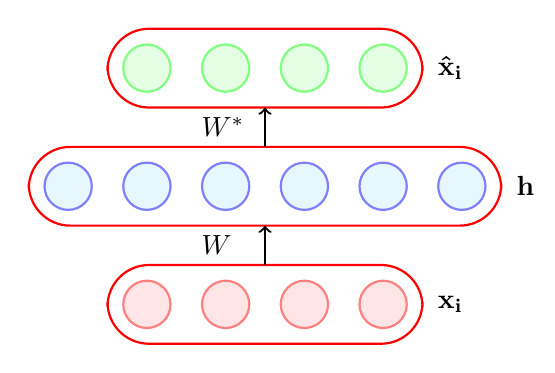
\begin{tikzpicture}

\node [input_neuron] (neuron01) at (8.5,4.5) {};
\node [input_neuron] (neuron02) at (9.5,4.5){};
\node [input_neuron] (neuron03) at (10.5,4.5) {};
\node [input_neuron] (neuron04) at (11.5,4.5) {};
\node [hidden_neuron] (neuron51) at (7.5,6) {} ;
\node [hidden_neuron] (neuron52) at (8.5,6)  {};
\node [hidden_neuron] (neuron53) at (9.5,6)  {};
\node [hidden_neuron] (neuron54) at (10.5,6)  {};
\node [hidden_neuron] (neuron55) at (11.5,6)  {};
\node [hidden_neuron] (neuron56) at (12.5,6)  {};

\node [output_neuron] (neuron11) at (8.5,7.5)  {};
\node [output_neuron] (neuron12) at (9.5,7.5)  {};
\node [output_neuron] (neuron13) at (10.5,7.5)  {};
\node [output_neuron] (neuron14) at (11.5,7.5)  {};


\node[text width=0.01cm] at (12.2,4.5) {$\mathbf{x_i}$};
\node[text width=0.007cm] at (9.2,5.25) {$W$};
\node[text width=0.01cm] at (13.2,6) {$\mathbf{h}$};
\node[text width=0.007cm] at (9.2,6.75) {$W^*$};
\node[text width=0.01cm] at (12.2,7.5) {$\mathbf{\hat{x}_i}$};

\draw[red!100,thick,solid,rounded corners=15pt] (8,4) rectangle (12,5);
\draw[red!100,thick,solid,rounded corners=15pt] (7,5.5) rectangle (13,6.5);
\draw[red!100,thick,solid,rounded corners=15pt] (8,7) rectangle (12,8);


\draw[thick,->] (10,5) -- (10,5.5);

\draw[thick,->] (10,6.5) -- (10,7);

\end{tikzpicture}
\end{center}
        }
    \end{overlayarea}
  \end{columns}
\end{frame}

\begin{frame}
  \begin{columns}
    \column{0.5\textwidth}
    \begin{overlayarea}{\textwidth}{\textheight}
        \begin{itemize}\justifying
            \item<1-> If the input has $n$ dimensions and the hidden layer has $k$ dimensions then
            \item<3-> In other words, the $(j,l)$ entry of the Jacobian captures the variation in the output of the $l^{th}$ neuron with a small variation in the $j^{th}$ input.
        \end{itemize}
    \end{overlayarea}

    \column{0.5\textwidth}
    \begin{overlayarea}{\textwidth}{\textheight}
    \only<2->{
        \[
            J_{\textbf{x}}(\mathbf{h}) = \begin{bmatrix}
                \frac{\partial{h_1}}{\partial{x_1}} & \dots & \dots & \dots &  \frac{\partial{h_1}}{\partial{x_n}} \\
                \frac{\partial{h_2}}{\partial{x_1}} & \dots & \dots & \dots & \frac{\partial{h_2}}{\partial{x_n}} \\
                \vdots & & \ddots & & \vdots \\
                \frac{\partial{h_k}}{\partial{x_1}} & \dots & \dots & \dots & \frac{\partial{h_k}}{\partial{x_n}}
            \end{bmatrix}
        \]
    }
    \only<4->{
        \[ 
            \|J_{\textbf{x}}(\mathbf{h})\|_F^2 = \sum_{j=1} ^n \sum_{l=1} ^k \bigg(\frac{\partial{h_l}}{\partial{x_j}}\bigg)^2
        \]
    }
    \end{overlayarea}
  \end{columns}
\end{frame}


\begin{frame}
\vspace{0.5cm}
\begin{columns}
    \column{0.5\textwidth}
    \begin{overlayarea}{\textwidth}{\textheight}
    \only<1->{
    \begin{itemize}\justifying
    \item<1-> What is the intuition behind this ?
    \item<2-> Consider $\frac{\partial h_1}{\partial x_1}$, what does it mean if 
          $\frac{\partial h_1}{\partial x_1} = 0$
    \item<3-> It means that this neuron is not very sensitive to variations in the 
          input $x_1$.
    \item<4-> But doesn't this contradict our other goal of minimizing $\mathcal{L} (\theta)$
          which requires $\mathbf{h}$ to capture variations in the input.
    \end{itemize}
    }
    \end{overlayarea}

    \column{0.5\textwidth}
    \begin{overlayarea}{\textwidth}{\textheight}
    \[
        \| J_{\textbf{x}}(\mathbf{h}) \|^2_F = \sum_{j=1}^{n} \sum_{l=1}^{k} 
                              \Big( \frac{\partial h_l}{\partial x_j} \Big)^2
    \]
    % \include{ae-approach}
    \input{modules/Module6/tikz_images/ae-approach.tex}
    \end{overlayarea}
\end{columns}
\end{frame}

\begin{frame}
\vspace{0.5cm}
\begin{columns}
    \column{0.5\textwidth}
    \begin{overlayarea}{\textwidth}{\textheight}
    \only<1->{
    \begin{itemize}\justifying
    \item<1-> Indeed it does and that's the idea
    \item<2-> By putting these two contradicting objectives against each other
          we ensure that $\textbf{h}$ is sensitive to only very important variations
          as observed in the training data.
    \item<3-> $\mathcal{L} (\theta)$ - capture important variations in data
    \item<4-> $\Omega (\theta)$ - do not capture variations in data
    \item<5-> Tradeoff - capture only very important variations in the data
    \end{itemize}
    }
    \end{overlayarea}

    \column{0.5\textwidth}
    \begin{overlayarea}{\textwidth}{\textheight}
    \[
        \| J_{\textbf{x}}(\mathbf{h}) \|^2_F = \sum_{j=1}^{n} \sum_{l=1}^{k} 
                              \Big( \frac{\partial h_l}{\partial x_j} \Big)^2
    \]
    % \include{ae-approach}
    \input{modules/Module6/tikz_images/ae-approach.tex}
    \end{overlayarea}
\end{columns}
\end{frame}

\begin{frame}
\begin{block}{}
Let us try to understand this with the help of an illustration.
\end{block}
\end{frame}
\begin{frame}

\begin{columns}
    \column{0.5\textwidth}
       \begin{overlayarea}{\textwidth}{\textheight}
       		
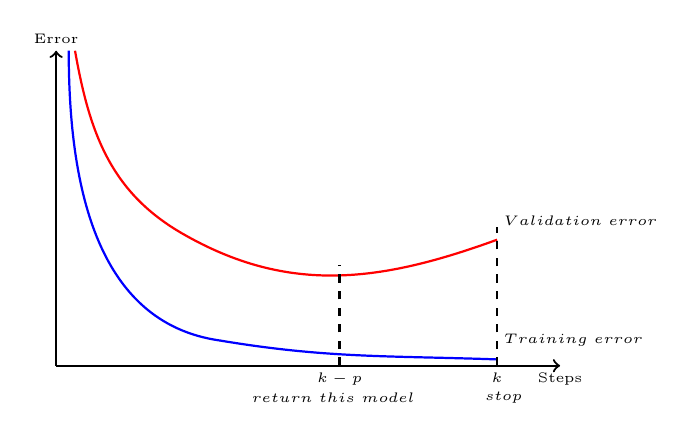
\begin{tikzpicture}[scale=0.8]
	\tiny
	\draw[thick,->] (0,0) -- (8,0) node [below] {Steps};
	\draw[thick,->] (0,0) -- (0,5) node [above] {Error};
	\draw[thick,blue] (0.2,5) to [out=270,in=172] (2.6,0.4);
	\draw[thick,blue] (2.6,0.4) to [out=350.5,in=178] (7,0.1);
	\node [right] at (7,0.4) {$Training$ $error$};
	\draw[thick,red] (0.3,5) to [out=280,in=150] (2,2.1);
	\draw[thick,red] (2,2.1) to [out=330,in=200] (7,2);
	%\draw[snake=sn[red]e]  (2,2.1) -- (7,2);
	\node [right] at (7,2.3) {$Validation$ $error$};
	\draw[thick,dashed] (4.5,0) node[below]{$k-p$}--(4.5,1.6);
	\draw[thick,dashed] (7,0) node[below]{$k$}--(7,2.2);
	\node [right] at (6.7,-0.5) {$stop$};
	\node [right] at (3,-0.5) {$return$ $this$ $model$};
	%\draw (0,2) to [out=340,in=200] (7,1.8);
	%\node [right] at (7,1.8) {$AVC$};
	%\draw (0,2) to [out=315,in=240] (7,5);
	%\node [right] at (7,5) {$MC$};
\end{tikzpicture}
    	\end{overlayarea}
    \column{0.5\textwidth}
    \begin{overlayarea}{\textwidth}{\textheight}
    \only<2->{
    \begin{itemize}\justifying
    \item<2-> Consider the variations in the data along directions $\mathbf{u}_1$
          and $\mathbf{u}_2$
    \item<3-> It makes sense to maximize a neuron to be sensitive to variations
          along $\mathbf{u}_1$
    \item<4-> At the same time it makes sense to inhibit a neuron from being sensitive to
          variations along $\mathbf{u}_2$ (as there seems to be small noise and unimportant for
          reconstruction)
    \item<5-> By doing so we can balance between the contradicting goals of good reconstruction
          and low sensitivity.
    \item<6-> What does this remind you of ?
    \end{itemize}
    }
    \end{overlayarea}
\end{columns}
\end{frame}

% Module 6: ends here (Slide 46 to 51)

